% Scribe template is a combination of 16831 and 10725. Thanks to those TAs!
\documentclass[11pt]{article}
\usepackage{latexsym}
\usepackage{amsmath}
\usepackage{amssymb}
\usepackage{amsthm}
\usepackage{bm}
\usepackage{epsfig}
\usepackage[tight]{subfigure}
\usepackage[framed,numbered,autolinebreaks,useliterate]{mcode}


\newcommand{\handout}[5]{
  \noindent
  \begin{center}
  \framebox{
    \vbox{
      \hbox to 5.78in { {#1} \hfill #2 }
      \vspace{4mm}
      \hbox to 5.78in { {\Large \hfill #5  \hfill} }
      \vspace{2mm}
      \hbox to 5.78in { {\em #3 \hfill #4} }
    }
  }
  \end{center}
  \vspace*{4mm}
}

\newcommand{\lecture}[5]{\handout{#1}{#2}{#3}{#4}{#5}}
\newcommand{\mat}[1]{\mathbf{#1}}

\newtheorem{theorem}{Theorem}
\newtheorem{corollary}[theorem]{Corollary}
\newtheorem{lemma}[theorem]{Lemma}
\newtheorem{observation}[theorem]{Observation}
\newtheorem{proposition}[theorem]{Proposition}
\newtheorem{definition}[theorem]{Definition}
\newtheorem{claim}[theorem]{Claim}
\newtheorem{fact}[theorem]{Fact}
\newtheorem{assumption}[theorem]{Assumption}

% 1-inch margins, from fullpage.sty by H.Partl, Version 2, Dec. 15, 1988.
\topmargin 0pt
\advance \topmargin by -\headheight
\advance \topmargin by -\headsep
\textheight 8.9in
\oddsidemargin 0pt
\evensidemargin \oddsidemargin
\marginparwidth 0.5in
\textwidth 6.5in

\parindent 0in
%\parskip 1.5ex
%\renewcommand{\baselinestretch}{1.25

\begin{document}
\newcommand{\defeq}[0]{\ensuremath{\stackrel{\triangle}{=}}}
\def\x{\mathbf{x}}
\def\w{\mathbf{w}}
\def\K{\mathbf{K}}
\lecture{{\bf 16-822}: Geometry-based Methods in Vision (F16) }{Released: Sep-19th. Due: Oct. 3rd. }{Lecturer: Martial Hebert}{TA: Nick Rhinehart}{Homework 1}


\section{Theory (45 Points)}

\subsection{$H$ for mirror reflection image (8 Points)}
Suppose that a scene is a plane and that it is projected to an image assuming
the normal pinhole model. Suppose that the points on the plane are related
by a symmetry about a line $L$ (for example, imagine a painting in which the
``left'' and ``right'' half are identical).
\begin{itemize}
\item Show that there exists a planar homography $H$ in the image such that
any point $p$ on the image matches other point $p' = Hp$ on the
image plane.
\item Show that $H^2 = I$.
\item Show that $H$ has an eigenvector which is the vanishing point of $L$.
\end{itemize}


\subsection{Fun with pencils of lines (12 Points)}

\begin{itemize}

\item A line in the plane is represented by a 3-vector $l = [u\ v\ w]^T$. What is the slope $s$ of the line? (Ignoring the one case of infinite slope)

\item Consider a pencil of lines in the plane. Explain why any line in the pencil can be represented canonically by a linear combination of two distinct
lines represented by two 3-vectors $l_1$ and $l_2$. (Simple answer, just use an argument based on the dimension of the subspaces involved.)

\item Now consider two pencils of lines and a homography $H$ between the two pencils. 
What is the dimension of the matrix representing $H$? (again, no equations; 
1-sentence answer based of the dimensions of the spaces involved) Be careful that we are asking about the homography from one set of lines to another, not about a planar homography.

\item  Show that if $l'$ is the transformed of $l$ by the line homography $H$, then the slopes 
are related by a function of the form (ignoring the infinities):
\begin{align*}
s' = \frac{as+b}{cs+d}
\end{align*}

\item Conversely, assume that a transformation between the two pencils is of that form, state what condition the coefficients $a,b,c,d$ must
satisfy for the transformation to be a line homography? What is the matrix representing that homography?
\end{itemize}

\subsection{Rodrigues's rotation formula (and some motion) (25 Points)}
\begin{itemize}

\item Rodrigues's rotation formula is a convenient way of expressing rotations of a vector $\mat{p}$ as 
a function of the rotation angle $\theta$ and the axis of rotation $\mat{w}$:
\begin{align*}
\mat{R}\mat{p} = \mat{p} + \sin(\theta) \mat{w} \times \mat{p} + (1 - \cos(\theta)) \mat{w} \times(\mat{w} \times \mat{p})
\end{align*}
Write Rodrigues's formula in matrix form:
\begin{align*}
\mat{R}\mat{p}=\ldots
\end{align*}
\item Suppose now that $\theta$ is very small (e.g., the small rotation between two consecutive frames in a video sequence). 
What would be an approximation of $\mat{RP}$, denoting $\mat{\omega} = \theta \mat{w}$?
\item Consider now 2 cameras separated by a small rotation $R$ and a translation $t$. Assuming $K=I$ (calibrated cameras) and using the approximation above, what is
the essential matrix $E$?

\item We know that the epipole in one image is $t$. What is the epipole in the 
other image if the axis of rotation $w$ is parallel to $t$?

\item Consider now a pixel of coordinates $(u,v)$ in one image, projection
of a point $(X,Y,Z)$. The corresponding point in the other image is $(u',v')$. 
Assuming again small motion we have: $u' = u + du$ and $v' = v + dv$ (we can
think of $du$ and $dv$ as the apparent motion of the point corresponding to $(u,v)$
in the image.)

Express $du$ and $dv$ as function of $u,v,\Omega,t,Z$ (remember to write first that $(u,v)$ are
the projection in the image of $X,Y,Z$ from the trivial projection matrix $[I\ 0]$.)

\item Show that if P is known to be on a plane $(n,d)$, then $(du,dv)$ does not depend on $Z$, the 
``depth'' of the point.

\item In that case, also show that $(du,dv)$ are quadratic expressions in $u,v$.

\item The reasoning above used derivatives ($du$ and $dv$). Another angle on the problem is to compute the homography $H$ induced by 
a plane $(n,d)$ assuming small rotation $\Omega$ and a translation $t$. Write an expression for $H$ using the 
small-angle rotation expression above.

\item Given this expression of $H$, which point remains invariant under $H$ if $\Omega$ is orthogonal to $n$? (e.g., if the plane is 
the ground plane and the cameras are on a robot moving on the ground plane).
\end{itemize}


\section{Having fun by implementing what we have learnt! (55 Points)}

In this part of the homework, we will try to generate metrically correct view of a warped image. You can use \underline{{\bf any method you prefer}} as long as it conforms to the descriptions below:
\\
\\
{\bf What you have to do:}\vspace{-0.25in}\\
\begin{itemize}
\item Given an example image, write a function that returns metrically rectified image as well as the $H$ used to perform rectification. Follow this function definition:\vspace{-0.05in}
$$\texttt{function [rectI, H] = rectifyImage(filename, debug)}\vspace{-0.05in}$$
If $\texttt{debug=1}$, you should provide whatever manual input (annotation) you require (e.g., marking parallel or perpendicular lines, planes etc.). $\texttt{MATLAB's ginput}$ might come in handy.\vspace{-0.05in}
$$\texttt{[x y] = ginput(4); pt1 = [x(1) y(1) 1]'; pt2 = [x(2) y(2) 1]';}\vspace{-0.05in}$$
Save all the information you entered, so that it can be evaluated. You can use any format for saving, as long as it is consistent with your load commands. \\
If $\texttt{debug=0}$, you should load whatever information you manually entered and return $\texttt{[rectI, H]}$. Follow this convention for saving/loading:\vspace{-0.05in}
\begin{align*}
&\texttt{[d, fname] = fileparts(filename);}\\
&\texttt{data = load(fullfile(strrep(d, `/images', `/data'), [fname `.mat']));}
\end{align*}
where $\texttt{fname.mat}$ is the file that stores the annotations (above code assumes images and annotated data are in $\texttt{`anypath/images/'}$ and $\texttt{`anypath/data/'}$ directories respectively.)
\item Capture (or find) {\bf 3} your own images. Ideally, capture/find images that have substantial perspective distortion. (See figure~\ref{fig:goodbad})
\item Run your code on at least {\bf 7 out of the given 13} images as well as on the images you captured/found. Put your images in the sub-folder $\texttt{./images/}$ and the $\texttt{mat}$ files with annotations in the sub-folder $\texttt{./data/}$.
\item See what you need to submit in the end.
\end{itemize}

\begin{figure}[h!]
\centering
\begin{subfigure}[Good input!]
{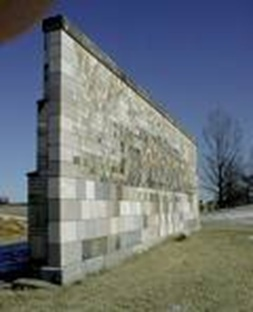
\includegraphics[width=0.2\textwidth]{tmpimages/good.jpg}}
\end{subfigure}
\begin{subfigure}[Bad input...]{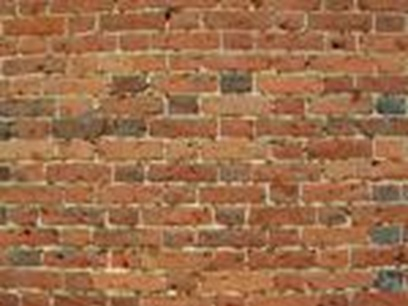
\includegraphics[width=0.3\textwidth, keepaspectratio=true]{tmpimages/bad.jpg}}
\end{subfigure}
\caption{The good and bad inputs.}
%\vspace{-0.2in}
\label{fig:goodbad}
\end{figure}

{\bf What you can use:}\vspace{-0.05in}
\begin{itemize}
\item You can use {\bf any method you prefer}. You might get ideas from material taught in class (16822) and Computer Vision (16720). Also, material from Hartley$\&$Zisserman, and Faugeras might be helpful. Any variations on the ideas for rectification mentioned in stated materials, e.g., there are other combinations of parallel/perpendicular points and lines, as well as methods using distances which Martial mentioned in class are fine.
\item You can also use advanced material from any papers/research/reports that you find, as long as you understand them.
\item Code to manually select points or planar regions in the image. (e.g., MATLAB’s ginput)
\item $\texttt{MATLAB}'$s functions or your code from 16720 used for warping. This might be helpful as well:
\vspace{-0.2in}
\lstinputlisting{applyH.m}
\item Non-linear distortion compensation code if the images you choose are too distorted. (Try not to choose such images).
\end{itemize}

{\bf What you {\it can not} do:}\vspace{-0.25in}\\
\begin{itemize}
\item Download code, except for the distortion and manual input (see above.)
\item Use any measurement in the scene provided apriori (the only information available as input is the image itself, and whatever you annotate).
\item Use any calibration parameters for the camera.
\item Make any assumption about the camera parameters, except that it is a perspective camera.
\end{itemize}


{\bf What you have to submit:}\vspace{-0.05in}
\begin{itemize}
\item Input images
\item Output images: Rectified image and intermediate images color coded annotation that you used. Display of the lines that were used, including the vanishing line if you use it in your method. (See figure~\ref{fig:ann})
\item Angles (more precisely, the cosines) of at least 3 pairs of perpendicular lines before and after rectification (provide annotations in the mat file as well). This will show how far from 0 the cosines are in the original image and how close to correct the final metric rectification is. (See figure~\ref{fig:cosines} and table~\ref{tab:cos}).
\item Description of your implementation (i.e., the algorithm you followed with relevant equations, what were the annotations used) and (most importantly) what problems were encountered (e.g., numerical issues, etc.).
\item {\bf CODE}.
\end{itemize}

\begin{figure}[h!]
\centering
\begin{subfigure}[Input images]
{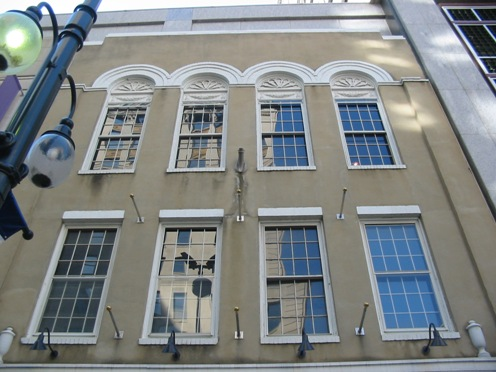
\includegraphics[width=0.23\textwidth]{tmpimages/facade.jpg}
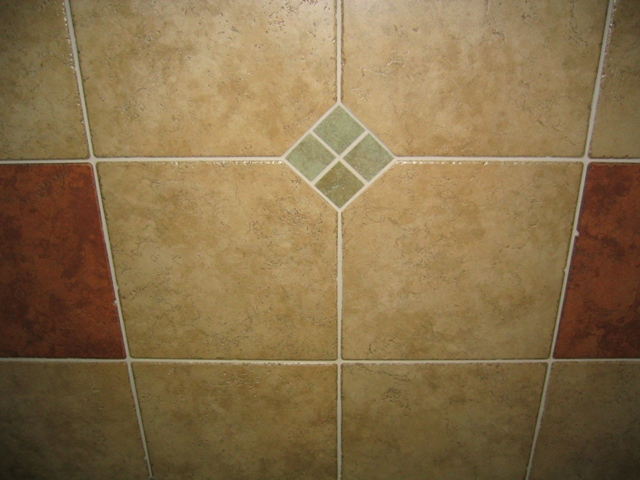
\includegraphics[width=0.23\textwidth]{tmpimages/tt2.jpg}
}
\end{subfigure}
\begin{subfigure}[Annotated $\|$ lines on input images]
{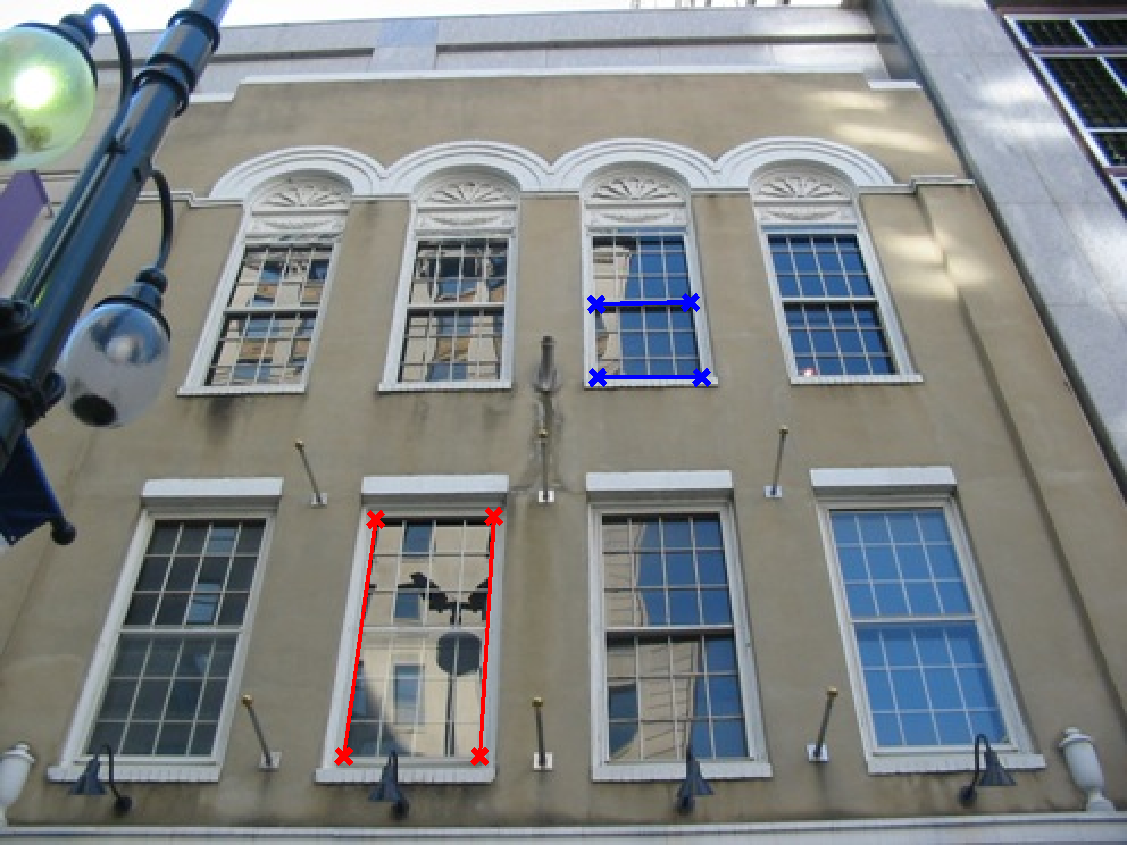
\includegraphics[width=0.23\textwidth]{tmpimages/facade-parallel-lines.png}
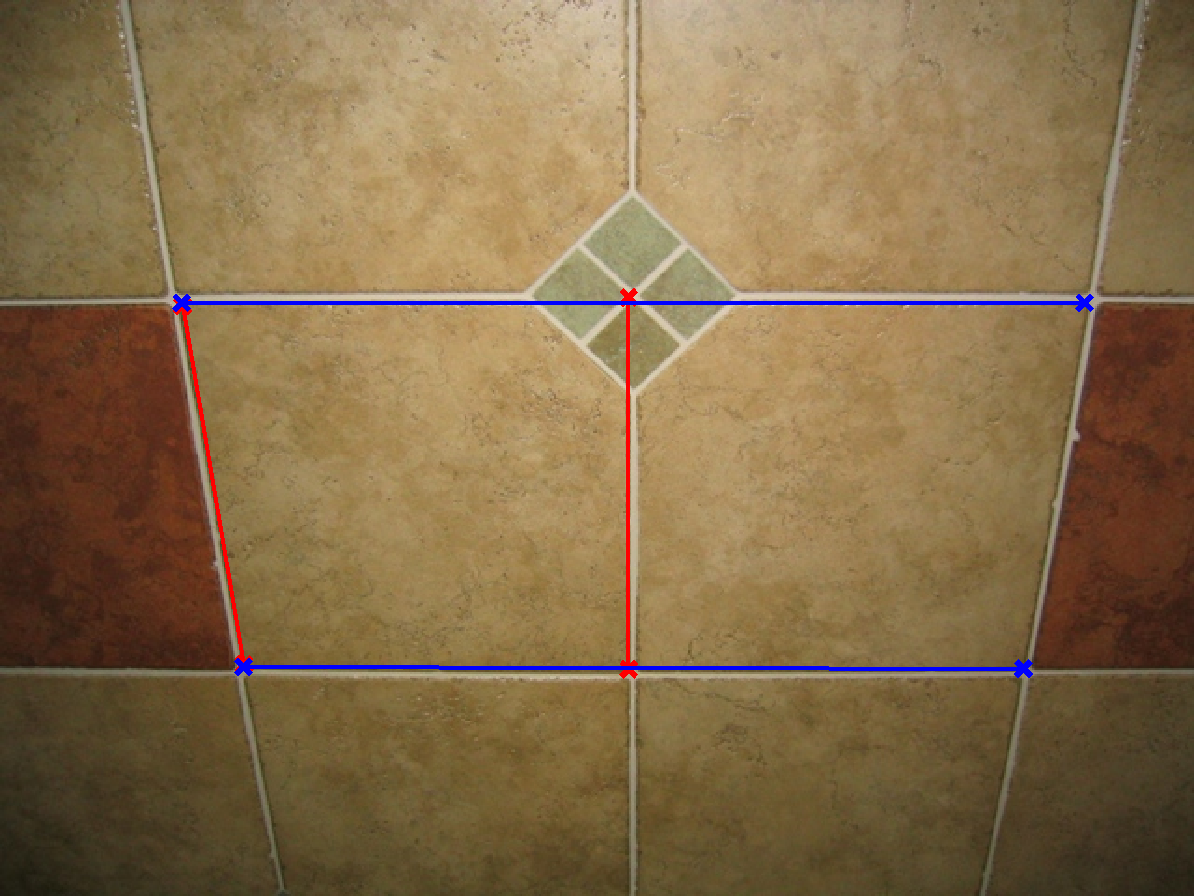
\includegraphics[width=0.23\textwidth]{tmpimages/tt2-parallel-lines.png}
}
\end{subfigure}
\begin{subfigure}[Annotated $\perp$ lines on affine rectified images]
{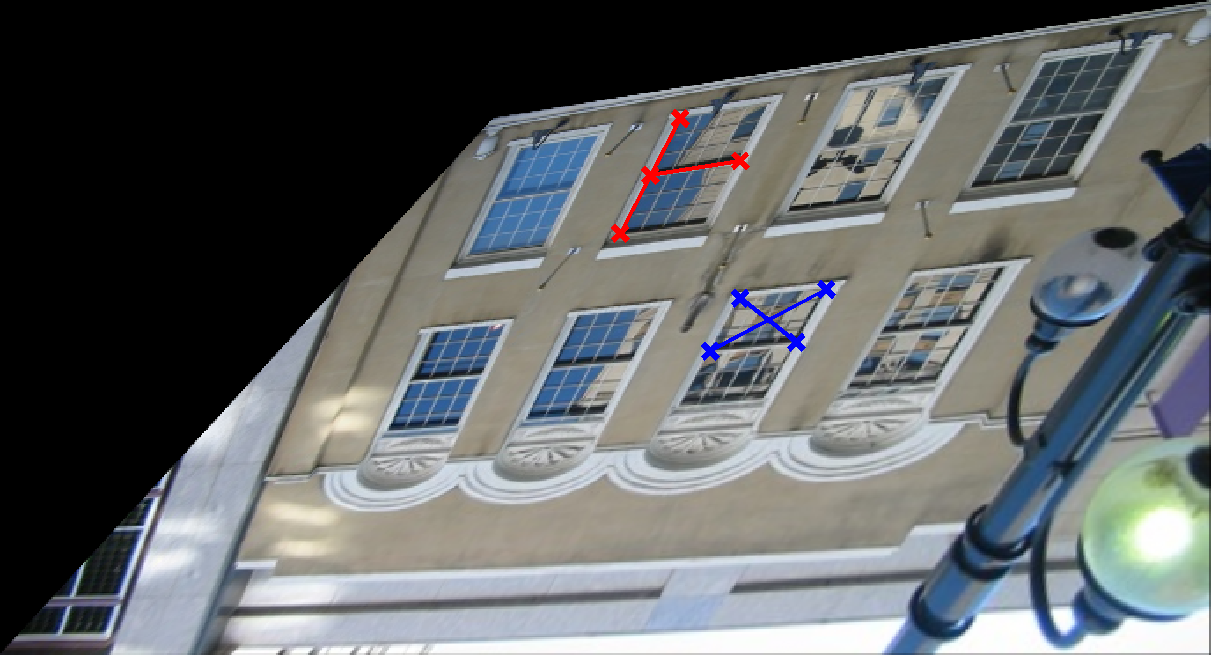
\includegraphics[width=0.23\textwidth]{tmpimages/facade-perpendicular-lines.png}
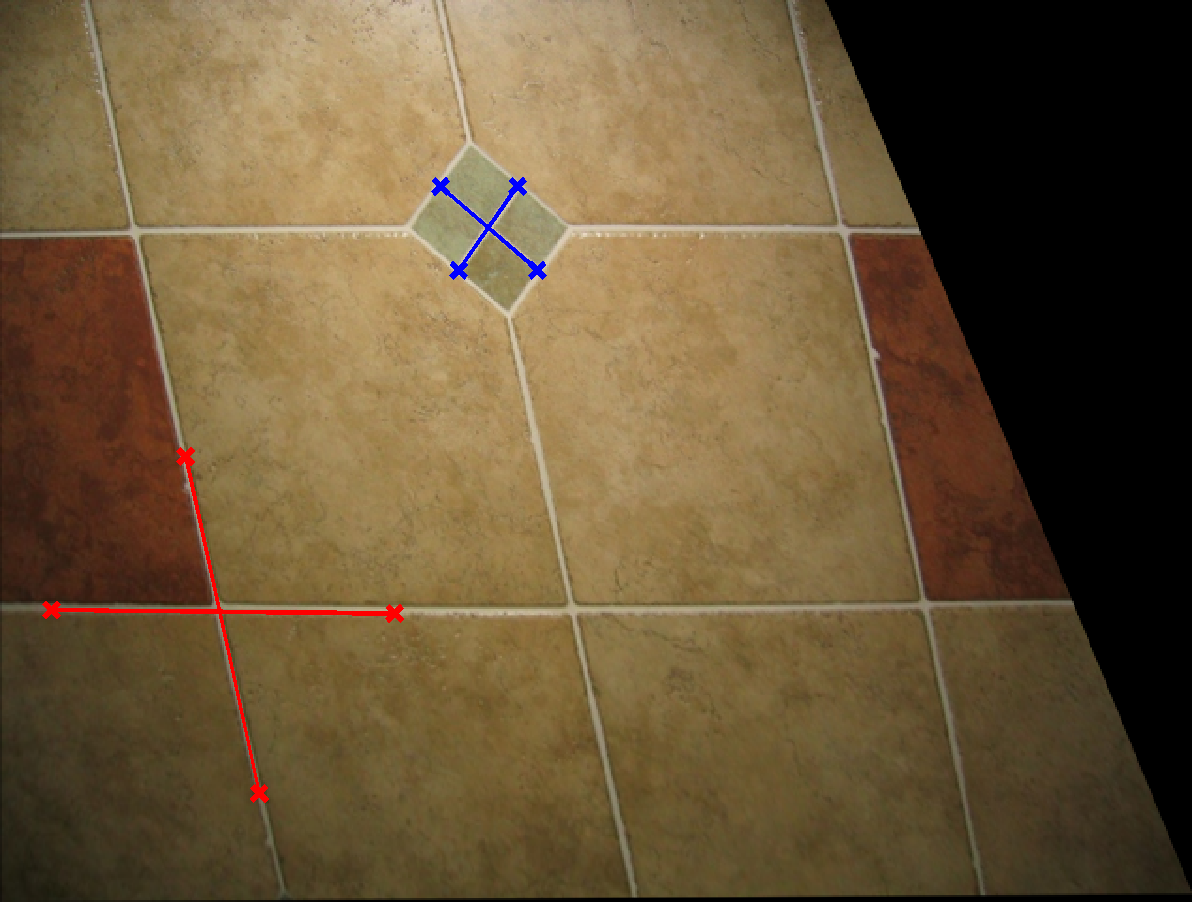
\includegraphics[width=0.23\textwidth]{tmpimages/tt2-perpendicular-lines.png}}
\end{subfigure}
\begin{subfigure}[Rectified image]
{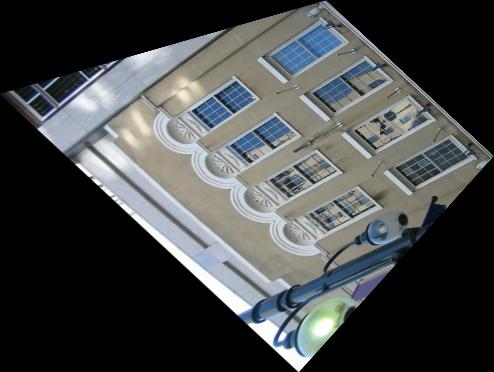
\includegraphics[width=0.23\textwidth]{tmpimages/facade-rect.jpg}
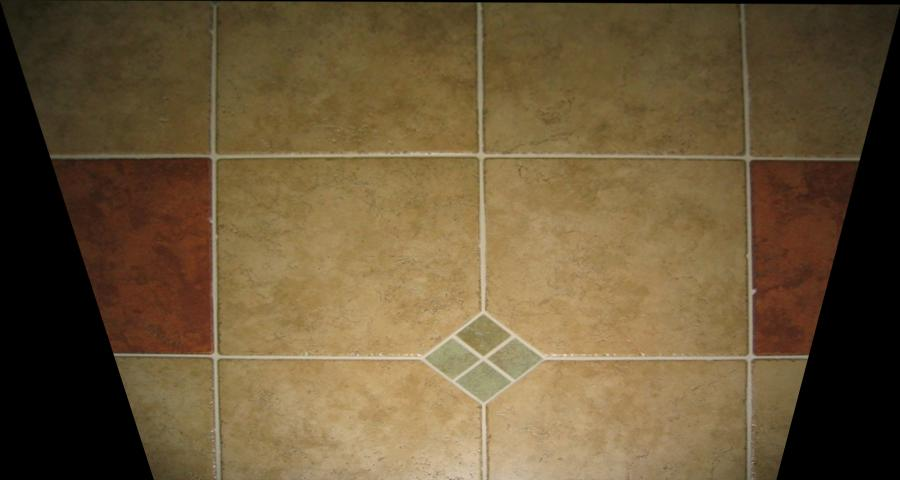
\includegraphics[width=0.23\textwidth]{tmpimages/tt2-rect.jpg}}
\end{subfigure}
\caption{An example of Output Images to be submitted for the rectification algorithm}
\label{fig:ann}
\end{figure}
%\clearpage
\begin{figure}[h!]
\centering
\begin{subfigure}[Input image]
{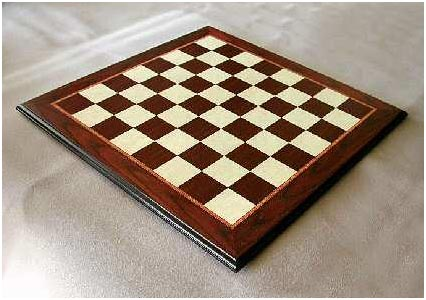
\includegraphics[width=0.3\textwidth]{tmpimages/chess2.jpg}}
\end{subfigure}
\begin{subfigure}[Annotated lines for which angles are computed]
{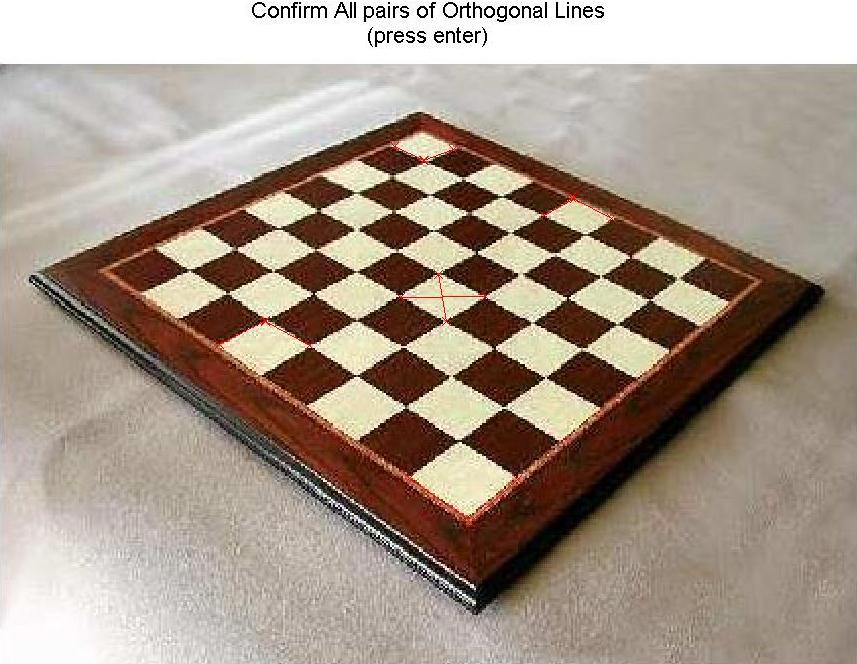
\includegraphics[width=0.3\textwidth]{tmpimages/chess2-lines.jpg}}
\end{subfigure}
\begin{subfigure}[Rectified Image]
{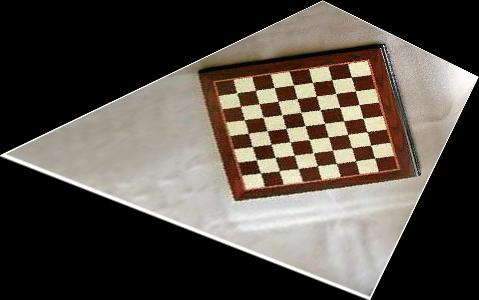
\includegraphics[width=0.3\textwidth]{tmpimages/chess2-rectified.jpg}}
\end{subfigure}
\caption{An example of Output Images to submit for angle between lines.}
\label{fig:cosines}
\end{figure}
\begin{table}[h!]
\centering
\begin{tabular}{|c|c|}
    \hline
  Before & After \\ \hline
-0.15073 & -0.00624 \\ \hline
0.10344 & 0.004659 \\ \hline
0.159543 & -0.001270 \\
    \hline
  \end{tabular}
  \caption{An example of cosine $\theta$ between lines.}
  \label{tab:cos}
  \end{table}

{\bf Tips:}
\begin{itemize}
\item Make sure to keep ``sanity checks'' in your code while you are debugging, by checking an equation that you know should be true. (e.g., $l^TCm=0$). Keep such code commented when you submit, so that I can see and appreciate it!
\item Nomalize coordinates of points before doing anything.
\item Remember the transformations that you are estimating are up to a scale.
\item Be careful about all the things Martial mentioned in class!
\item Have fun!!
\end{itemize}

\end{document}
